\documentclass[11pt,a4paper]{article}

\usepackage[margin=2.5cm]{geometry}
\usepackage{booktabs}
\usepackage{longtable}
\usepackage{array}
\usepackage{float}
\usepackage{amsmath}
\usepackage{pgfplots}
\pgfplotsset{compat=1.18}

\title{Experimental Study of Sorting Algorithm Performance}
\author{Maria Maiorescu \\[4pt]
\small{Year 1, Computer Science} \\
\small{West University of Timișoara}}
\date{\today}

\begin{document}

\maketitle

\begin{abstract}
This paper compares six sorting algorithms implemented in C: bubble sort, quick sort, insertion sort, selection sort, merge sort, and radix sort. The code in \texttt{algorithms.c} generates integer arrays with different patterns and measures average sorting time. The measured values are taken from \texttt{results.csv}. We compare theoretical Big-O complexity predictions with empirically measured results.
\end{abstract}

\section{Introduction}
Sorting is one of the most common tasks in computer science. Different sorting algorithms have different speeds and behave differently depending on the input \cite{cormen2009,sedgewick2011}. The goal of this study is to analyze how algorithm type and input pattern affect running time.

The study analyzes:
\begin{itemize}
    \item algorithm category (\(O(n^2)\), \(O(n\log n)\), and radix-based),
    \item input size,
    \item input variant (reversed, random, and partially sorted).
\end{itemize}

\section{Experimental Setup}
The experiment is implemented in \texttt{algorithms.c}. For each test case, the program creates a new integer array, sorts it, measures the time with \texttt{clock()}, and then frees the memory.

\subsection{Algorithms}
The following algorithms are implemented:
\begin{itemize}
    \item \textbf{bubble sort}: compares neighbors and swaps them if needed; easy to understand, but slow for big arrays,
    \item \textbf{quick sort} (last element as pivot): splits the array around a pivot and sorts the two parts,
    \item \textbf{insertion sort}: builds a sorted part from left to right by inserting each new element,
    \item \textbf{selection sort}: repeatedly finds the smallest value and puts it in the next correct position,
    \item \textbf{merge sort}: splits the array into smaller parts, sorts them, then merges them,
    \item \textbf{radix sort} (base-10 counting by digit): sorts integers digit by digit.
\end{itemize}

These algorithms were chosen because they use different ideas, so we can compare both theory and real measured performance.

\subsection{Input Data Generation}
The program generates integer arrays in these variants:
\begin{itemize}
    \item \textbf{reversed}: strictly descending sequence,
    \item \textbf{random}: uniformly generated integers in \([0, n]\),
    \item \textbf{partially sorted}: initially sorted sequence followed by random swaps.
\end{itemize}

For partially sorted arrays, factors \(10\%, 30\%, 50\%, 70\%, 90\%\) are used in the labels. Higher percentages mean the array is closer to already sorted.

\subsection{Sizes and Number of Runs}
The exact experiment configuration used in \texttt{main()} is:
\begin{itemize}
    \item \(n=10\), runs \(=1{,}000{,}000\)
    \item \(n=50\), runs \(=1{,}000{,}000\)
    \item \(n=100\), runs \(=1{,}000{,}000\)
    \item \(n=1000\), runs \(=100\)
    \item \(n=10000\), runs \(=10\)
    \item \(n=100{,}000\), runs \(=1\)
    \item \(n=1{,}000{,}000\), runs \(=1\) (partial; execution stopped after bubble sort due to a stack overflow crash)
\end{itemize}

The reported values are average elapsed time in milliseconds.

\section{Theoretical Complexity (Big-O)}
Table~\ref{tab:complexity} summarizes expected complexity based on standard algorithm analysis \cite{cormen2009,knuth1998}.

Big-O tells us how the running time should grow when \(n\) gets larger. The measured times show what happens in practice, including effects from implementation details such as pivot choice and memory allocation.

\begin{table}[H]
\centering
\begin{tabular}{>{\raggedright\arraybackslash}p{3cm}ccc>{\raggedright\arraybackslash}p{3cm}}
\toprule
Algorithm & Best & Average & Worst & Extra Space \\
\midrule
Bubble Sort & \(O(n)\) & \(O(n^2)\) & \(O(n^2)\) & \(O(1)\) \\
Insertion Sort & \(O(n)\) & \(O(n^2)\) & \(O(n^2)\) & \(O(1)\) \\
Selection Sort & \(O(n^2)\) & \(O(n^2)\) & \(O(n^2)\) & \(O(1)\) \\
Quick Sort & \(O(n\log n)\) & \(O(n\log n)\) & \(O(n^2)\) & \(O(\log n)\) stack \\
Merge Sort & \(O(n\log n)\) & \(O(n\log n)\) & \(O(n\log n)\) & \(O(n)\) \\
Radix Sort & \(O(d(n+b))\) & \(O(d(n+b))\) & \(O(d(n+b))\) & \(O(n+b)\) \\
\bottomrule
\end{tabular}
\caption{Theoretical complexity comparison. Here, \(d\) is number of digits and \(b\) is base/range per digit pass.}
\label{tab:complexity}
\end{table}

\section{Experimental Results from \texttt{results.csv}}
The next tables present measured average times (ms), split by algorithm type, input variant, and input size: bubble sort (Table~\ref{tab:bubble-results}), quick sort (Table~\ref{tab:quick-results}), insertion sort (Table~\ref{tab:insertion-results}), selection sort (Table~\ref{tab:selection-results}), merge sort (Table~\ref{tab:merge-results}), and radix sort (Table~\ref{tab:radix-results}).

\subsection{Bubble Sort}
\begin{table}[H]
\centering
\footnotesize
\begin{tabular}{lcccccc}
\toprule
Variant & 10 & 50 & 100 & 1000 & 10000 & 100000 \\
\midrule
reversed & 0.001 & 0.010 & 0.037 & 3.711 & 361.338 & 13228.117 \\
random & 0.001 & 0.013 & 0.047 & 3.120 & 310.295 & 18520.945 \\
partially sorted 10\% & 0.001 & 0.007 & 0.027 & 2.537 & 254.257 & 9423.954 \\
partially sorted 30\% & 0.001 & 0.004 & 0.020 & 2.353 & 245.054 & 8105.251 \\
partially sorted 50\% & 0.001 & 0.004 & 0.017 & 2.264 & 236.306 & 7537.942 \\
partially sorted 70\% & 0.001 & 0.004 & 0.013 & 2.176 & 232.797 & 7643.391 \\
partially sorted 90\% & 0.001 & 0.004 & 0.013 & 2.169 & 230.022 & 7640.430 \\
\bottomrule
\end{tabular}
\caption{Bubble sort average elapsed time (ms) by input variant and size.}
\label{tab:bubble-results}
\end{table}

\begin{table}[H]
\centering
\begin{tabular}{lc}
\toprule
Variant & 1{,}000{,}000 \\
\midrule
reversed & 1{,}318{,}479 \\
random & 1{,}808{,}240 \\
partially sorted 10\% & 929{,}435 \\
partially sorted 30\% & 794{,}225 \\
partially sorted 50\% & 756{,}972 \\
partially sorted 70\% & 738{,}981 \\
partially sorted 90\% & 722{,}408 \\
\bottomrule
\end{tabular}
\caption{Bubble sort at \(n=1{,}000{,}000\): average elapsed time (ms). This was a single run. All remaining algorithms crashed before completing at this size (see Section~\ref{sec:notes}).}
\label{tab:bubble-1m}
\end{table}

Bubble sort's \(O(n^2)\) scaling is clearly visible: at \(n=100{,}000\) random input takes over 18 seconds, and at \(n=1{,}000{,}000\) it took over 30 minutes (Table~\ref{tab:bubble-1m}). The early-exit optimisation helps on partially sorted data but does not change the fundamental growth rate. After bubble sort completed at \(n=1{,}000{,}000\), the program crashed with a segmentation fault — the remaining algorithms were not measured at this size.

\subsection{Quick Sort}
\begin{table}[H]
\centering
\footnotesize
\begin{tabular}{lcccccc}
\toprule
Variant & 10 & 50 & 100 & 1000 & 10000 & 100000 \\
\midrule
reversed & 0.001 & 0.010 & 0.036 & 3.215 & 312.116 & 12725.631 \\
random & 0.001 & 0.005 & 0.011 & 0.160 & 2.140 & 10.412 \\
partially sorted 10\% & 0.001 & 0.007 & 0.015 & 0.217 & 3.103 & 14.681 \\
partially sorted 30\% & 0.001 & 0.010 & 0.028 & 0.367 & 5.100 & 17.405 \\
partially sorted 50\% & 0.001 & 0.010 & 0.032 & 0.622 & 9.882 & 41.464 \\
partially sorted 70\% & 0.001 & 0.010 & 0.037 & 0.780 & 7.438 & 50.374 \\
partially sorted 90\% & 0.001 & 0.010 & 0.037 & 1.052 & 10.578 & 72.064 \\
\bottomrule
\end{tabular}
\caption{Quick sort average elapsed time (ms) by input variant and size.}
\label{tab:quick-results}
\end{table}

Quick sort is very fast on random input, which matches the expected average \(O(n\log n)\) time. But it is much slower on reversed and nearly ordered inputs. The gap is extreme at \(n=100{,}000\): 10.412 ms (random) vs. 12725.631 ms (reversed) — almost as slow as bubble sort. The reason is the last-element pivot, which creates maximally uneven splits on sorted or reversed input, leading to \(O(n^2)\) behaviour.

\subsection{Insertion Sort}
\begin{table}[H]
\centering
\footnotesize
\begin{tabular}{lcccccc}
\toprule
Variant & 10 & 50 & 100 & 1000 & 10000 & 100000 \\
\midrule
reversed & 0.001 & 0.007 & 0.025 & 2.385 & 235.495 & 8343.083 \\
random & 0.001 & 0.005 & 0.015 & 1.209 & 118.386 & 4198.798 \\
partially sorted 10\% & 0.001 & 0.002 & 0.005 & 0.292 & 27.537 & 985.757 \\
partially sorted 30\% & 0.001 & 0.001 & 0.002 & 0.109 & 9.985 & 342.495 \\
partially sorted 50\% & 0.001 & 0.001 & 0.002 & 0.069 & 6.381 & 222.384 \\
partially sorted 70\% & 0.001 & 0.001 & 0.001 & 0.052 & 4.604 & 165.761 \\
partially sorted 90\% & 0.001 & 0.001 & 0.001 & 0.042 & 3.688 & 122.072 \\
\bottomrule
\end{tabular}
\caption{Insertion sort average elapsed time (ms) by input variant and size.}
\label{tab:insertion-results}
\end{table}

Insertion sort's sensitivity to input order is even more visible at \(n=100{,}000\): 4198.798 ms on random input compared to only 122.072 ms on 90\% partially sorted. This confirms the near-linear best case when few elements are out of place.

\subsection{Selection Sort}
\begin{table}[H]
\centering
\footnotesize
\begin{tabular}{lcccccc}
\toprule
Variant & 10 & 50 & 100 & 1000 & 10000 & 100000 \\
\midrule
reversed & 0.001 & 0.006 & 0.023 & 2.093 & 206.273 & 7143.945 \\
random & 0.001 & 0.009 & 0.031 & 2.388 & 230.297 & 6847.988 \\
partially sorted 10\% & 0.001 & 0.007 & 0.026 & 2.347 & 233.828 & 6856.536 \\
partially sorted 30\% & 0.001 & 0.007 & 0.026 & 2.345 & 239.237 & 6747.636 \\
partially sorted 50\% & 0.001 & 0.007 & 0.026 & 2.345 & 235.613 & 6656.085 \\
partially sorted 70\% & 0.001 & 0.007 & 0.025 & 2.346 & 235.761 & 6655.227 \\
partially sorted 90\% & 0.001 & 0.007 & 0.026 & 2.363 & 234.586 & 6765.990 \\
\bottomrule
\end{tabular}
\caption{Selection sort average elapsed time (ms) by input variant and size.}
\label{tab:selection-results}
\end{table}

Selection sort has similar times for all input variants of the same size. This is expected because it always scans the remaining unsorted part to find the minimum. Its running time increases strongly with \(n\), as expected for \(O(n^2)\).

\subsection{Merge Sort}
\begin{table}[H]
\centering
\begin{tabular}{lcccccc}
\toprule
Variant & 10 & 50 & 100 & 1000 & 10000 & 100000 \\
\midrule
reversed & 0.001 & 0.005 & 0.010 & 0.124 & 1.481 & 20.611 \\
random & 0.001 & 0.007 & 0.016 & 0.214 & 2.778 & 28.249 \\
partially sorted 10\% & 0.001 & 0.005 & 0.012 & 0.150 & 1.928 & 23.177 \\
partially sorted 30\% & 0.001 & 0.005 & 0.011 & 0.138 & 1.709 & 22.078 \\
partially sorted 50\% & 0.001 & 0.005 & 0.010 & 0.135 & 1.671 & 22.141 \\
partially sorted 70\% & 0.001 & 0.005 & 0.010 & 0.129 & 1.685 & 21.452 \\
partially sorted 90\% & 0.001 & 0.005 & 0.010 & 0.130 & 1.660 & 21.385 \\
\bottomrule
\end{tabular}
\caption{Merge sort average elapsed time (ms) by input variant and size.}
\label{tab:merge-results}
\end{table}

Merge sort has stable times across variants, with small differences between random, reversed, and partially sorted inputs. This is consistent with \(O(n\log n)\). It scales well compared to quadratic algorithms.

\subsection{Radix Sort}
\begin{table}[H]
\centering
\begin{tabular}{lcccccc}
\toprule
Variant & 10 & 50 & 100 & 1000 & 10000 & 100000 \\
\midrule
reversed & 0.001 & 0.003 & 0.005 & 0.066 & 0.856 & 5.932 \\
random & 0.001 & 0.003 & 0.007 & 0.103 & 1.010 & 6.419 \\
partially sorted 10\% & 0.001 & 0.003 & 0.005 & 0.087 & 0.913 & 5.705 \\
partially sorted 30\% & 0.001 & 0.003 & 0.005 & 0.065 & 0.926 & 5.299 \\
partially sorted 50\% & 0.001 & 0.003 & 0.005 & 0.065 & 0.855 & 5.285 \\
partially sorted 70\% & 0.001 & 0.003 & 0.005 & 0.066 & 0.866 & 5.440 \\
partially sorted 90\% & 0.001 & 0.003 & 0.005 & 0.067 & 0.851 & 5.236 \\
\bottomrule
\end{tabular}
\caption{Radix sort average elapsed time (ms) by input variant and size.}
\label{tab:radix-results}
\end{table}

Radix sort is the fastest in most medium and large tests. Since it sorts integers digit by digit, its time is close to linear for these value ranges. Input order matters less than for comparison-based sorts.

\subsection{Overall Comparison}

Figure~\ref{fig:comparison-random} plots all six algorithms on random input using a log--log scale, making it easy to see how sharply the $O(n^2)$ group diverges from the efficient algorithms as $n$ grows.

\begin{figure}[H]
\centering
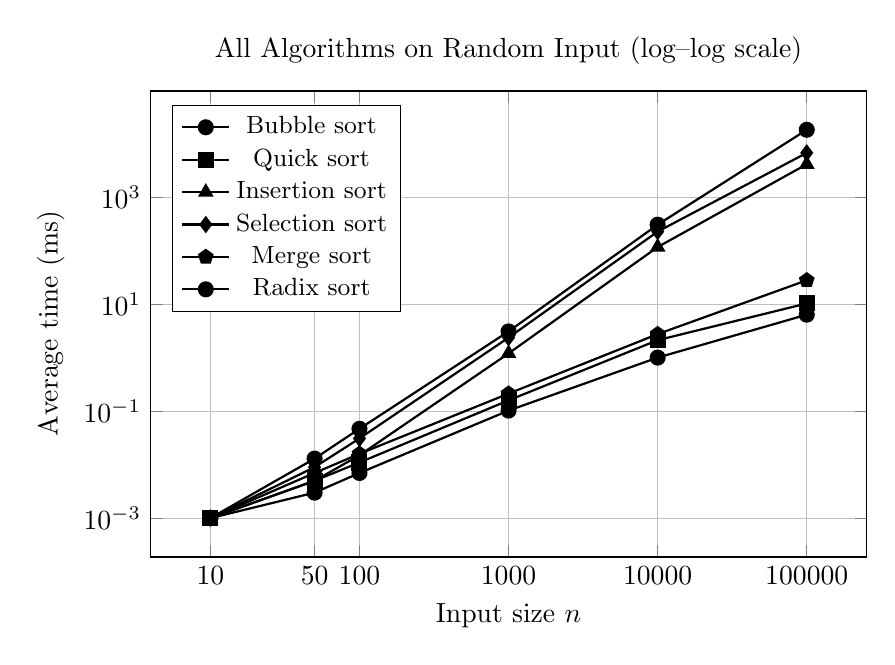
\begin{tikzpicture}
\begin{loglogaxis}[
    width=0.88\textwidth,
    height=7.5cm,
    xlabel={Input size $n$},
    ylabel={Average time (ms)},
    xtick={10,50,100,1000,10000,100000},
    xticklabels={10,50,100,1000,10000,100000},
    legend pos=north west,
    legend style={font=\small},
    grid=major,
    mark size=2.5pt,
    title={All Algorithms on Random Input (log--log scale)}
]
\addplot[mark=*,thick]                  coordinates {(10,0.001)(50,0.013)(100,0.047)(1000,3.120)(10000,310.295)(100000,18520.945)};
\addlegendentry{Bubble sort}
\addplot[mark=square*,thick]            coordinates {(10,0.001)(50,0.005)(100,0.011)(1000,0.160)(10000,2.140)(100000,10.412)};
\addlegendentry{Quick sort}
\addplot[mark=triangle*,thick]          coordinates {(10,0.001)(50,0.005)(100,0.015)(1000,1.209)(10000,118.386)(100000,4198.798)};
\addlegendentry{Insertion sort}
\addplot[mark=diamond*,thick]           coordinates {(10,0.001)(50,0.009)(100,0.031)(1000,2.388)(10000,230.297)(100000,6847.988)};
\addlegendentry{Selection sort}
\addplot[mark=pentagon*,thick]          coordinates {(10,0.001)(50,0.007)(100,0.016)(1000,0.214)(10000,2.778)(100000,28.249)};
\addlegendentry{Merge sort}
\addplot[mark=otimes*,thick]            coordinates {(10,0.001)(50,0.003)(100,0.007)(1000,0.103)(10000,1.010)(100000,6.419)};
\addlegendentry{Radix sort}
\end{loglogaxis}
\end{tikzpicture}
\caption{Average elapsed time (ms) vs.\ input size $n$ for all six algorithms on random input (log--log scale). The $O(n^2)$ algorithms (bubble, insertion, selection) diverge steeply, while merge sort and radix sort remain fast at large $n$.}
\label{fig:comparison-random}
\end{figure}

\section{Discussion: Expected vs. Observed Behavior}
\subsection{Main Trends}
The results confirm the expected classes of behavior:
\begin{itemize}
    \item Bubble, insertion, and selection sorts get slow quickly as \(n\) grows, as expected for \(O(n^2)\) (Tables~\ref{tab:bubble-results}, \ref{tab:insertion-results}, and \ref{tab:selection-results}).
    \item Merge sort stays fast and stable for all variants, matching \(O(n\log n)\) (Table~\ref{tab:merge-results}).
    \item Radix sort is the fastest in this integer experiment, with near-linear behavior (Table~\ref{tab:radix-results}).
\end{itemize}

\subsection{Input Variant Sensitivity}
\begin{itemize}
    \item Insertion sort strongly benefits from partially sorted data. At \(n=10{,}000\): 118.386 ms (random) vs. 3.688 ms (90\% sorted). At \(n=100{,}000\): 4198.798 ms (random) vs. 122.072 ms (90\% sorted) — see Table~\ref{tab:insertion-results}.
    \item Selection sort changes very little across variants because it always does almost the same work (Table~\ref{tab:selection-results}).
    \item Quick sort is sensitive to reversed and nearly sorted data in this implementation (Table~\ref{tab:quick-results}).
\end{itemize}

Figure~\ref{fig:insertion-variants} illustrates the effect of input ordering on insertion sort at $n=10{,}000$ in more detail.

\begin{figure}[H]
\centering
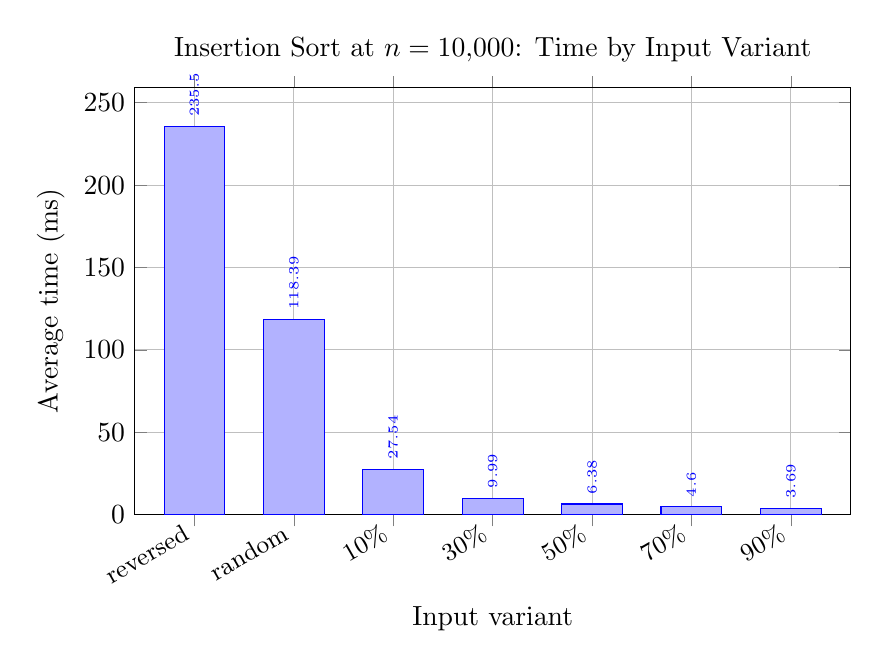
\begin{tikzpicture}
\begin{axis}[
    ybar,
    width=0.88\textwidth,
    height=7cm,
    xlabel={Input variant},
    ylabel={Average time (ms)},
    symbolic x coords={reversed, random, 10\%, 30\%, 50\%, 70\%, 90\%},
    xtick=data,
    x tick label style={rotate=30, anchor=east, font=\small},
    nodes near coords,
    every node near coord/.append style={font=\tiny, rotate=90, anchor=west},
    bar width=22pt,
    grid=major,
    ymin=0,
    title={Insertion Sort at $n=10{,}000$: Time by Input Variant}
]
\addplot coordinates {
    (reversed,  235.495)
    (random,    118.386)
    (10\%,       27.537)
    (30\%,        9.985)
    (50\%,        6.381)
    (70\%,        4.604)
    (90\%,        3.688)
};
\end{axis}
\end{tikzpicture}
\caption{Insertion sort average elapsed time (ms) at $n=10{,}000$ for each input variant. The percentage label indicates the degree of pre-sortedness of the array (higher = more sorted). The time drops dramatically as the array becomes more ordered, confirming the $O(n)$ best-case behaviour.}
\label{fig:insertion-variants}
\end{figure}

\subsection{Why Quick Sort Degrades Here}
In \texttt{algorithms.c}, quick sort uses the \emph{last element} as pivot. For sorted or reversed arrays, this always picks the worst possible pivot, creating maximally uneven splits and \(O(n^2)\) behaviour. This gap grows with \(n\): at \(n=10{,}000\): 2.140 ms (random) vs. 312.116 ms (reversed); at \(n=100{,}000\): 10.412 ms (random) vs. 12725.631 ms (reversed). At \(n=1{,}000{,}000\) the recursion stack would be one million levels deep, which is why the program crashed.

\subsection{Measurement Notes}\label{sec:notes}
For very small arrays (\(n=10,50,100\)), many values are near timer precision (often 0.001 ms), so small differences are not very reliable. For larger arrays (\(n=1{,}000\) to \(n=100{,}000\)) the trends are clear and consistent with theory. The \(n=100{,}000\) and \(n=1{,}000{,}000\) runs used a single trial (runs\,=\,1) rather than an average, so those values carry more measurement noise.

At \(n=1{,}000{,}000\), only bubble sort produced results. After it finished, the program crashed with a segmentation fault (exit code 139). The most likely cause is stack overflow in quick sort's recursive implementation: with the last-element pivot on the reversed or sorted input that follows bubble sort in the test sequence, the recursion depth reaches \(n\), which overflows the default 8\,MB system stack on macOS.

\section{Conclusion}
This study shows that practical performance follows theoretical complexity in most cases:
\begin{itemize}
    \item \(O(n^2)\) algorithms are acceptable only for small inputs.
    \item Merge sort and radix sort are reliable and fast for larger inputs.
    \item Quick sort can be very fast on random input but can become slow on ordered input with a simple pivot choice.
\end{itemize}

Choosing a sorting algorithm should therefore depend on both \textbf{input size} and \textbf{input pattern}. A better pivot strategy for quick sort (such as a random or median-of-three pivot) would make its performance more consistent across input types.

\begin{thebibliography}{9}

\bibitem{cormen2009}
Thomas H. Cormen, Charles E. Leiserson, Ronald L. Rivest, and Clifford Stein.
\textit{Introduction to Algorithms}.
3rd ed., MIT Press, 2009.

\bibitem{knuth1998}
Donald E. Knuth.
\textit{The Art of Computer Programming, Volume 3: Sorting and Searching}.
2nd ed., Addison-Wesley, 1998.

\bibitem{sedgewick2011}
Robert Sedgewick and Kevin Wayne.
\textit{Algorithms}.
4th ed., Addison-Wesley, 2011.

\end{thebibliography}

\end{document}